\documentclass[11pt]{article}
\usepackage[margin=1in, top=1in]{geometry}
\usepackage[all]{nowidow}
\usepackage[hyperfigures=true, hidelinks, pdfhighlight=/N]{hyperref}
\usepackage[separate-uncertainty=true, group-digits=false]{siunitx}
\usepackage{graphicx,amsmath,physics,tabto,float,amssymb,pgfplots,verbatim,tcolorbox}
\usepackage{listings,xcolor,caption,import,wrapfig,subcaption,biblatex,multirow,booktabs}
\usepackage[version=4]{mhchem}
\usepackage[noabbrev]{cleveref}
\newcommand{\creflastconjunction}{, and\nobreakspace}
\newcommand{\mb}[1]{\mathbf{#1}}
\numberwithin{equation}{section}
\numberwithin{figure}{section}
\numberwithin{table}{section}
\definecolor{stringcolor}{HTML}{C792EA}
\definecolor{codeblue}{HTML}{2162DB}
\definecolor{commentcolor}{HTML}{4A6E46}
\captionsetup{font=small, belowskip=0pt}
\lstdefinestyle{appendix}{
    basicstyle=\ttfamily\footnotesize,commentstyle=\color{commentcolor},keywordstyle=\color{codeblue},
    stringstyle=\color{stringcolor},showstringspaces=false,numbers=left,upquote=true,captionpos=t,
    abovecaptionskip=12pt,belowcaptionskip=12pt,language=Python,breaklines=true,frame=single}
\lstdefinestyle{inline}{
    basicstyle=\ttfamily\footnotesize,commentstyle=\color{commentcolor},keywordstyle=\color{codeblue},
    stringstyle=\color{stringcolor},showstringspaces=false,numbers=left,upquote=true,frame=tb,
    captionpos=b,language=Python}
\renewcommand{\lstlistingname}{Appendix}
\pgfplotsset{compat=1.17}
\addbibresource{bibliography.bib}

\begin{document}

\begin{center}
    {\huge Training a neural net to identify top quark jets}\\
    \vspace{0.2in}
    \textbf{KDSMIL001 | September 2022}    
    
    \begin{abstract}
        We train a neural net to identify jets as originating from top quarks as opposed to other quarks; a process known as top tagging. High-level variables describing the jets are used as opposed to constituent data as constituent requires considerably more computing power. The model's performance is then assessed according to some commonly used statistics and investigated for different $p_\mathrm{T}$ cuts.
    \end{abstract}
\end{center}

\section{Introduction}\label{sec:Introduction}
In proton-proton collisions at the Large Hadron Collider (LHC) at CERN, top quarks (along with their anti-particle counterpart) are produced about once every few seconds. Due to their proportionally large mass ($\sim\SI{173}{\giga\electronvolt}$) their decay time is too short for them to be observed directly, so the next best way to determine if a top quark was produced is to look at the hadronic jets produced by the interaction and determine if they were a result of a top quark or some other, less interesting quark. This process is called top-tagging.

One way to perform this classification between signal (top quark jet) and background (any other jet) is to use a neural net. Neural nets are well suited to this task as they are able to handle the large volumes of Monte Carlo truth data that are available to us and can easily be constructed to provide an output from 0 to 1, which we can take to be the neural net's classification of signal (closer to 1) and background (closer to 0). We used data from \url{https://cds.cern.ch/record/2825328}~\cite{top-tagging-data} to train and test a deep neural net in top-tagging using ``high-level'' quantities describing the jets. This report will focus on the creation of that neural net, its performance according to the confusion matrix, and some investigation into where the neural net performs best in relation to the kinematics of the jets being tagged.

\section{The data}\label{sec:Data}
The data we used to train and test the neural net comes from the dataset used in \cite{top-tagging-data}. It contains an equal number of background and signal jets. Due to computation power restrictions, we were unable to use their train dataset, so we split the test dataset into $\frac 23$ for training and $\frac 13$ for testing.

The data is split up into two types: constituent and high-level. The constituent data is simply the $p_\mathrm{T}$, $\eta$, $\varphi$ and energy $E$ of the particles making up each jet. This is a lot of information and would ultimately be the best data to use as it holds all the available information about a jet, which neural nets are very good at sifting through to find the information relevant to the task at hand. The only issue is that it takes a lot of RAM to load all the data into, as well as requiring a lot of computation power (or time) to really get to a meaningful result. 

To try cut down on computation time and resources, we used the high-level data. These are 15 variables calculated for each jet, from the constituent data, which have been identified by \cite{ATL-PHYS-PUB-2021-028} and \cite{ATL-PHYS-PUB-2017-004} as summarising the data in a way that lends itself to top-tagging. The 15 variables are:

\begin{itemize}
    \item Energy Correlation Ratios: $ECF_1,\; ECF_2,\; ECF_3,\; C_2,\; D_2$
    \item N-subjettiness: $\tau_1,\; \tau_2,\; \tau_3,\; \tau_4$
    \item Splitting Measures: $\sqrt{d_{12}},\; \sqrt{d_{23}}$
    \item Centre of Mass Observable: $\mathrm{Thrust}_\mathrm{MAJ}$
    \item $Q_W$, $L_2$, and $L_3$
\end{itemize}

Some preprocessing was needed to prepare the data for the training. If we were to use two input variables with wildly different scales, say energy on the \si[]{\giga\electronvolt} scale and distance on the nanometre scale, then changing an energy parameter even slightly will have such a large impact on the output of the neural net, and thus the loss function, that changing a distance parameter will practically have no effect. To avoid this, we did some basic preprocessing which involved simply subtracting the mean for a specific quantity from the value for all the jets, then dividing by the standard deviation. This centers the data around 0 and gives it a standard deviation of 1. Doing this ensures that our neural net will not be trained to weight a specific input more simply because it's on a larger scale than another input.

Each jet has a label stating whether it is signal or background, as well as weights used in training to re-weight the background so that its $p_\mathrm{T}$ distribution is the same as that of the signal. This is done since the production of the background events requires an unphysical $p_\mathrm{T}$ spectrum, so they could either be re-weighted according to the spectrum observed at the LHC, or they could be weighted to be identical to the signal distribution. The latter was chosen in order to avoid the neural net falsely tagging a signal jet as background simply because the training dataset didn't have any signal jets at that $p_\mathrm{T}$ due to them not being generated. 

The 15 high-level quantities, the labels, and the weights are all that we gave to the neural net for training.

\section{Creation and training of the neural net}\label{sec:CreatingNeuralNet}
The neural net was created using Python and Keras~\cite{keras}, which is an interface for using TensorFlow. We used an input layer with 15 inputs; one for each of the high-level quantities. We then used 3 hidden layers each with 20 neurons using the Rectified Linear Unit activation function. Finally, an output layer of 1 neuron using the sigmoid activation function was used to give us a prediction of signal (closer to 1) or background (closer to 0). The model was compiled with the argument \texttt{optimizer=`adam'}, which has a learning rate of 0.001. We used a batch size of 100, with our training set being made up of around 1.6 million jets. 8 epochs were used. A validation dataset of 5\% of the training dataset was used.

This configuration was chosen fairly arbitrarily, aside from the input and output layers, with a focus on simplicity and short run times (around 10 minutes of training). We chose the binary cross-entropy for our loss function as it is both simple and well-suited to a (who could've guessed it) binary classification task such as this one.

We can look at the evolution of the model with two parameters---the loss function and the accuracy---evaluated at each epoch in \cref{fig:loss_accuracy} for both the training and validation datasets. In this case, the accuracy is defined as the proportion of correct predictions when calling everything with prediction greater than 0.5 a signal, and background otherwise. This is a fairly rudimentary statistic and will be improved upon in later sections.

The neural net finished training with a loss function value of \num{0.3500} and an accuracy of \num{0.8442}.

\begin{figure}[h]%
    \centering
    \begin{subfigure}{.49\linewidth}
        \centering
        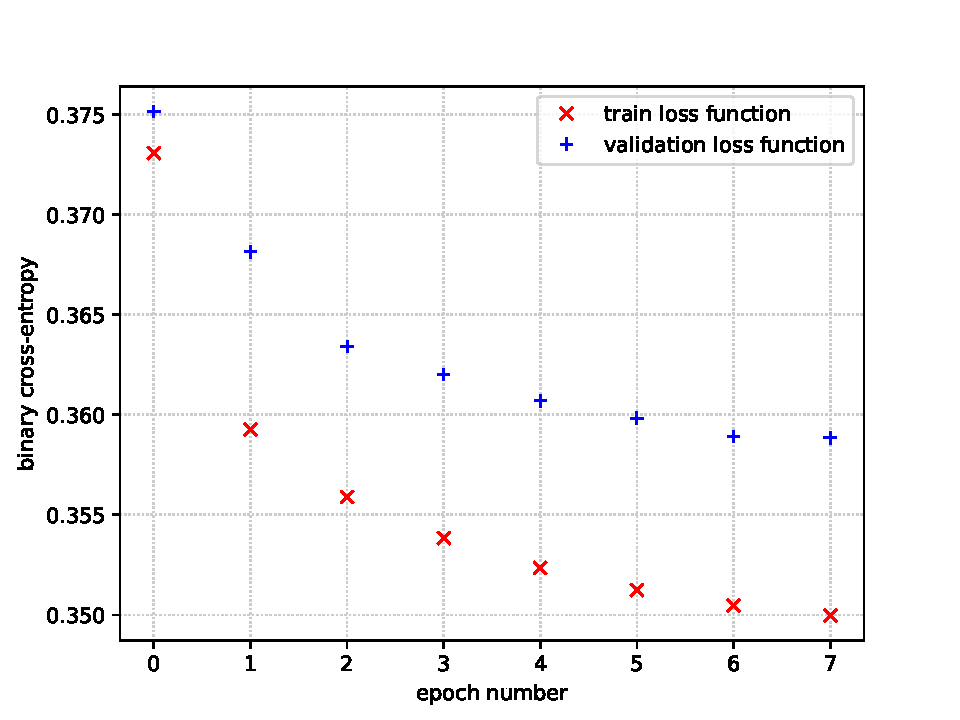
\includegraphics[width=\linewidth]{Plots/loss_history.pdf}
        \caption{Progression of the loss function over the training of the neural net, shown for both the training dataset as well as the validation dataset. The loss function used was binary cross-entropy.}
        \label{fig:loss_history}
    \end{subfigure}
    \hfill
    \begin{subfigure}{.49\linewidth}
        \centering
        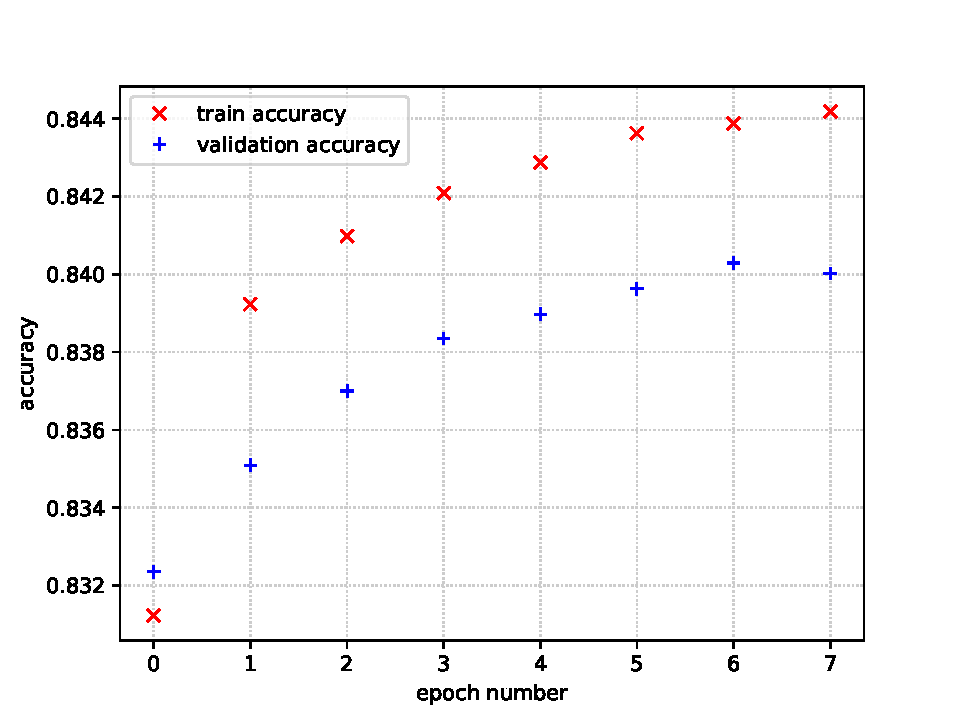
\includegraphics[width=\linewidth]{Plots/accuracy_history.pdf}
        \caption{Progression of the accuracy of the neural net over its training, evaluated on both the training dataset and the validation dataset. Accuracy here is defined simply as the proportion of correct predictions.}
        \label{fig:accuracy_history}
    \end{subfigure}
    \caption{}
    \label{fig:loss_accuracy}
\end{figure}

\section{Predictions and neural net performance}\label{sec:Predictions}
With the neural net trained, we were then able to use it to predict the classification of jets in our testing set. This dataset contained around 8 million jets. All predictions greater than 0.5 were considered signal and all less than or equal to 0.5 were considered background. A first step towards improving the accuracy metric calculated earlier is to look at the confusion matrix, which tells us how many true positives (TP), false negatives (FN), false positives (FP), and true negatives (TN) were predicted. In our case we are considering signal to be ``positive'' and background ``negative''.

\begin{table}[h]
    \centering
    \begin{tabular}{cccc}
        \multicolumn{2}{c}{\multirow{2}{*}{}} & \multicolumn{2}{c}{Predicted Classification} \\ \cmidrule{3-4}
        \multicolumn{2}{c}{} & Signal & Background \\ \cmidrule(lr){3-3} \cmidrule(lr){4-4}
        \multirow{2}{*}{Actual Classification} & Signal & 367092 & 42453 \\ \cmidrule(lr){2-2}
        & Background & 80269 & 329945 \\ \cmidrule(lr){2-2}
    \end{tabular}
    \caption{Confusion matrix for the predictions made by our neural net. Calculated using \texttt{sklearn.metrics.confusion\_matrix} with signal (1) considered positive and background (0) considered negative. Going row by row, each entry is the number of true positives, false negatives, false positives, and true negatives~\cite{Confusion_Matrix}}
    \label{tbl:conf_matrix}
\end{table}

\Cref{tbl:conf_matrix} shows the confusion matrix for our neural net, with an overall accuracy of 0.85030. From the values shown, we can calculate some useful quantities that describe the predictive power of the neural net. The first two are simply the true positive and true negative rates. They are found with $\mathrm{TPR}=\frac{\mathrm{TP}}{\mathrm{TP}+\mathrm{FN}}$ and $\mathrm{TNR}=\frac{\mathrm{TN}}{\mathrm{TN}+\mathrm{FP}}$. These are the proportions of true signal or background jets that were correctly identified as such, but this time the two classes are not mixed up so we can compare the neural net's ability to predict signal and background.

Next we can consider the positive and negative predictive values. These are defined as $\mathrm{PPV}=\frac{\mathrm{TP}}{\mathrm{TP}+\mathrm{FP}}$ and $\mathrm{NPV}=\frac{\mathrm{TN}}{\mathrm{TN}+\mathrm{FN}}$ and can be thought of as the proportion of, say, positive predictions that the neural net makes which are actually true positives. These statistics are subtly different to the TPR and TNR as they tell us how often a certain prediction is correct, as opposed to how often a certain true value is predicted correctly. The PPV is often called the precision, while the TPR can be thought of as an accuracy. 

We find these values to be 

\begin{equation*}
    \mathrm{TPR}=0.89634,\;\;\;\; \mathrm{TNR}=0.80432,\;\;\;\; \mathrm{PPV}=0.82057,\;\;\mathrm{and}\;\; \mathrm{NPV}=0.88600.
\end{equation*}

These tell us a few things. Firstly, our neural net is more likely (around 9\%) to correctly identify a signal event as signal than it is to identify a background event as background. We also see that when our neural net predicts a jet to be background, it is about 6\% more likely to be correct than when it predicts a jet to be signal. 

These two statements seem to be at odds with each other but they are in fact saying similar things. The higher TPR tells us that a true signal jet is less likely to be labelled as background than a background jet is to be labelled as signal. Similarly, the higher NPV tells us that if a jet is labelled as background, it is less likely that the jet is actually signal than a jet labelled signal is to actually be background. In other words, our neural net yields a more pure background distribution than it does for signal. 

For a visual representation of the distribution of signal and background events, we can plot a histogram of true signal and background events according to their prediction from the neural net. \Cref{fig:bkg_vs_signal} shows this. 

\begin{figure}[h]
    \begin{center}
        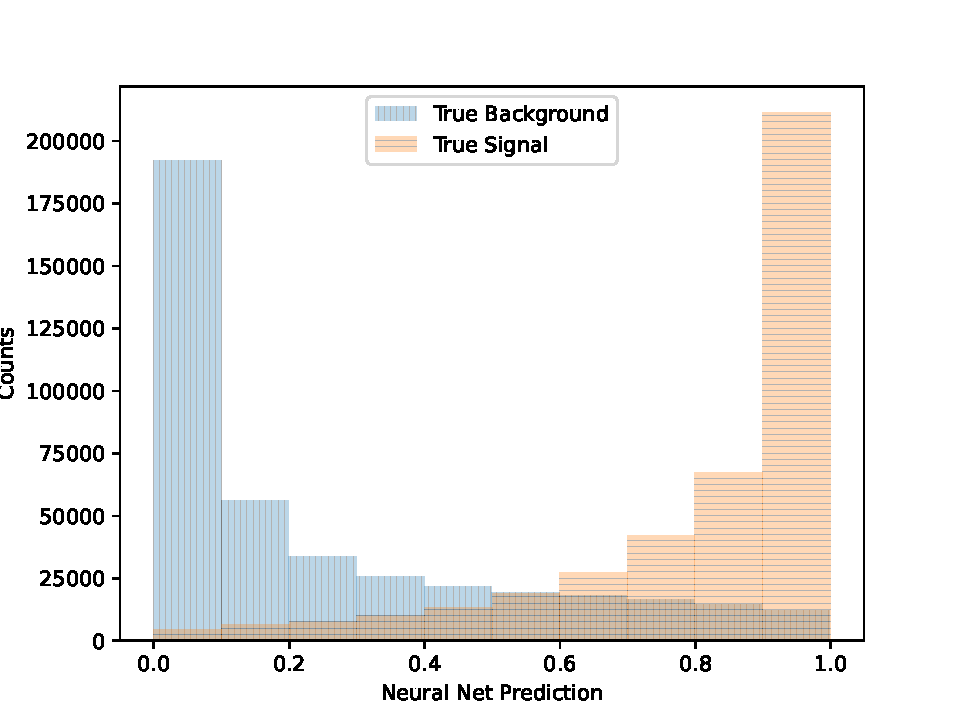
\includegraphics[width=.8\textwidth]{Plots/bkg_vs_signal.pdf}
        \caption{Histograms of true signal and background events, binned according to the prediction made by the neural net. Note that counts are not weighted according to the training weights as there are an equal number of signal and background events already and the weighting was only needed for dealing with the $p_\mathrm{T}$ distributions.}
        \label{fig:bkg_vs_signal}
    \end{center}
\end{figure}

We can see qualitatively from \cref{fig:bkg_vs_signal} that there are more true background events predicted as signal than signal events predicted as background, which is exactly what the TPR, TNR, PPV, and NPV told us before. The plot otherwise looks fairly symmetrical and gives us a good indication that there isn't anything wildly wrong with our neural net. From this plot, we could decide on a first approximation to a best cut to make on the prediction from the neural net, to decide whether something is a signal or background. Changing the cut from 0.5 to something like 0.8 would serve to remove much of the background jets from our signal sample, making it far more pure. This would, however, lead to many signal events being classified as background, so our overall accuracy would go down. Similarly, cutting at 0.2 would make a more pure background sample. So there are trade-offs to be made when deciding on the cut that are influenced by the intended use of the neural net.

\subsection{Performance in different kinematic regions}\label{sec:Kinematic_Performance}
Another way that we can evaluate the performance of the neural net is to look at how it performs with respect to, say, the $p_\mathrm{T}$ of the jets it classifies. 

\begin{figure}[h]%
    \centering
    \begin{subfigure}[t]{.49\linewidth}
        \centering
        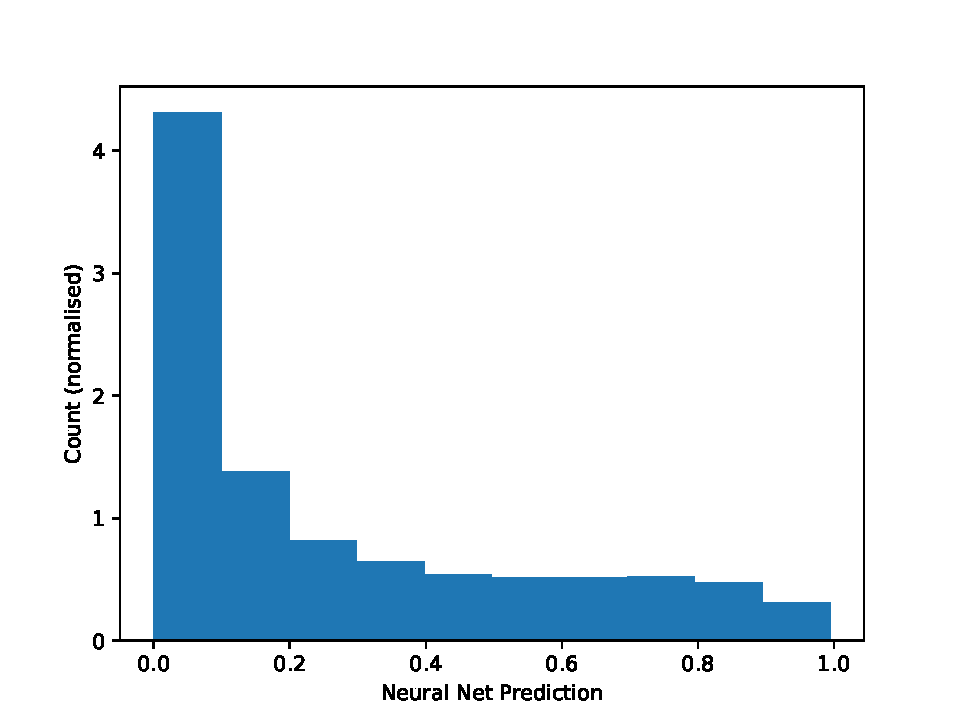
\includegraphics[width=\linewidth]{Plots/bkg_high_pt.pdf}
        \caption{Histogram of neural net predictions of background events in the high $p_\mathrm{T}$ region.}
        \label{fig:bkg_high_pt}
    \end{subfigure}
    \hfill
    \begin{subfigure}[t]{.49\linewidth}
        \centering
        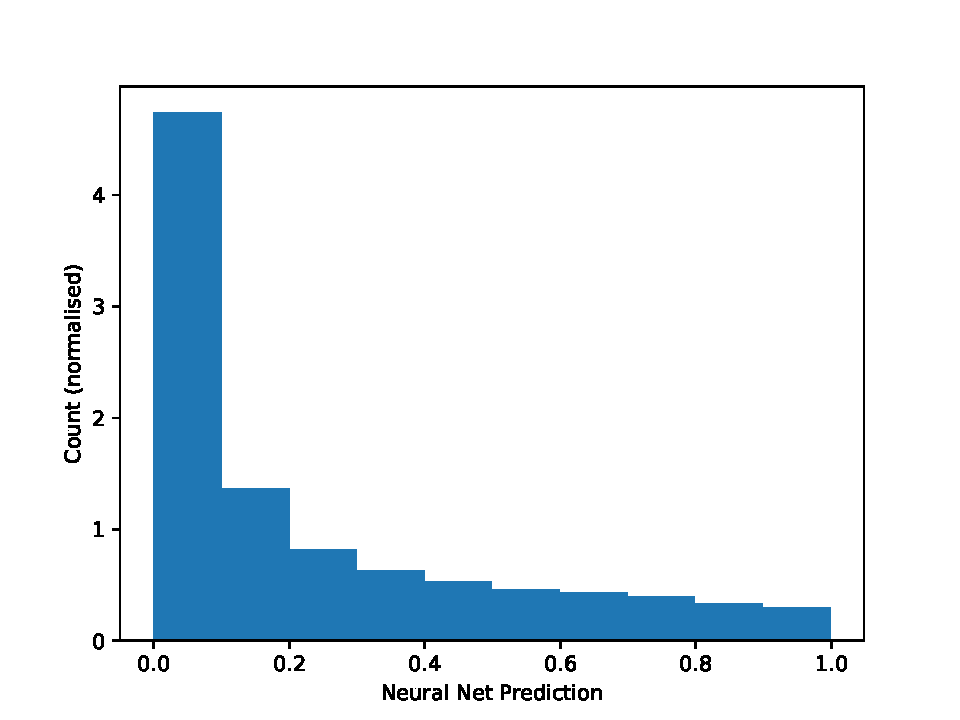
\includegraphics[width=\linewidth]{Plots/bkg_low_pt.pdf}
        \caption{Histogram of neural net predictions of background events in the low $p_\mathrm{T}$ region.}
        \label{fig:bkg_low_pt}
    \end{subfigure}
\caption{}
\label{fig:bkg_high_low}
\end{figure}

\begin{figure}[h]%
    \centering
    \begin{subfigure}[t]{.49\linewidth}
        \centering
        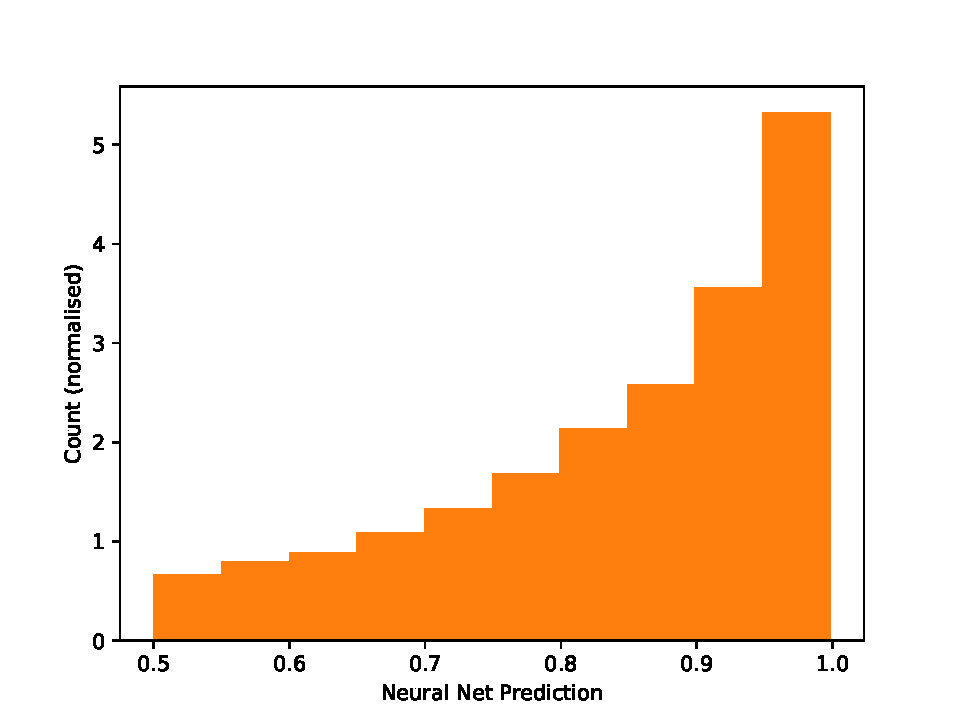
\includegraphics[width=\linewidth]{Plots/sig_high_pt.pdf}
        \caption{Histogram of neural net predictions of signal events in the high $p_\mathrm{T}$ region.}
        \label{fig:sig_high_pt}
    \end{subfigure}
    \hfill
    \begin{subfigure}[t]{.49\linewidth}
        \centering
        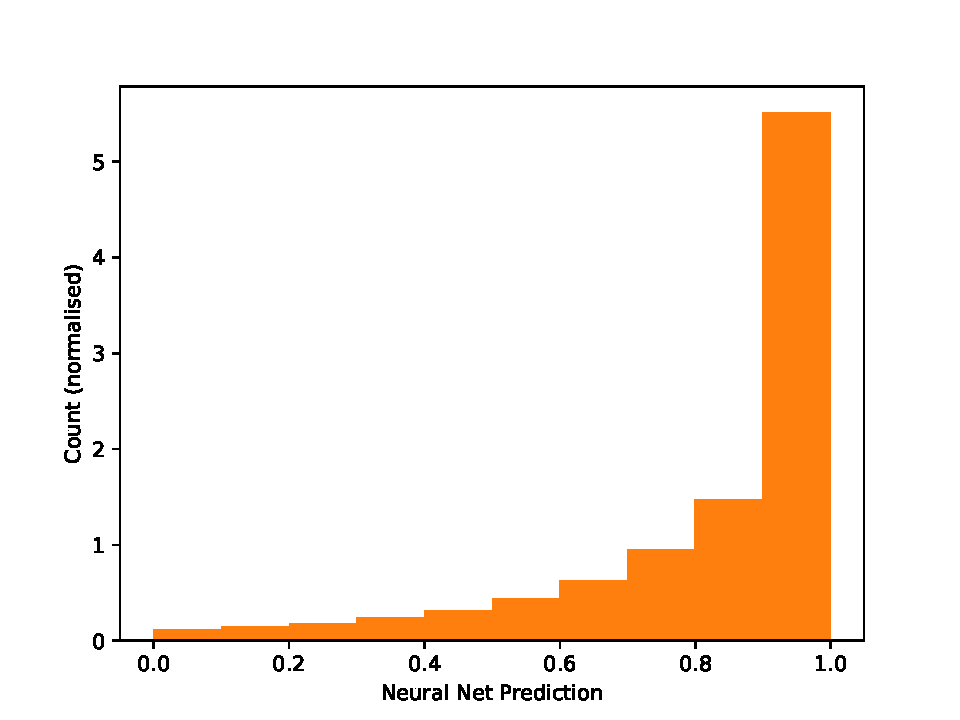
\includegraphics[width=\linewidth]{Plots/sig_low_pt.pdf}
        \caption{Histogram of neural net predictions of signal events in the high $p_\mathrm{T}$ region.}
        \label{fig:sig_low_pt}
    \end{subfigure}
\caption{}
\label{fig:sig_high_low}
\end{figure}

\Cref{fig:bkg_high_low,fig:sig_high_low} show histograms for the true background and signal jets, binned according to their neural net prediction. We have divided the two groups again by their $p_\mathrm{T}$ where low $p_\mathrm{T}$ is simply below the midpoint between the highest and lowest $p_\mathrm{T}$, and high $p_\mathrm{T}$ is above that. The histograms have been normalised for easier comparison as there are more low $p_\mathrm{T}$ events than high. 

We can see from the histograms that our neural net seems to perform a bit better at low $p_\mathrm{T}$ as the histograms for both background and signal are more sharply peaked than their high $p_\mathrm{T}$ counterparts. For a more quantitative view of this, we found the PPV, NPV, and overall accuracy of each $p_\mathrm{T}$ region:

\begin{table}[H]
    \centering
    \begin{tabular}{c|c|c}
         & Low $p_\mathrm{T}$ & High $p_\mathrm{T}$  \\ \hline
        PPV & 0.79325 & 0.90893 \\ 
        NPV & 0.90757 & 0.72474 \\
        ACC & 0.84928 & 0.85484
    \end{tabular}
\end{table}

We can see that the accuracy doesn't actually change appreciably, perhaps even favouring high $p_\mathrm{T}$ to some degree. What is interesting is that for low $p_\mathrm{T}$ the neural net performs in a similar fashion to how it performs on the whole, regarding the PPV and NPV, but for high $p_\mathrm{T}$ it seems to flip. This would mean that at high $p_\mathrm{T}$ the neural net is actually better at producing a pure signal sample than background. 

This is a curious result as there doesn't seem to be any reason for the neural net to perform differently in different kinematic regions, but investigating the nature and cause of this phenomenon is outside the scope of this report. 

\section{Conclusion}\label{sec:Conclusion}


\newpage
\printbibliography


\end{document}